\chapter{Anonimizzazione VS Pseudonimizzazione}

Anonimizzazione e pseudonimizzazione sono tecniche utilizzate per proteggere l'identità degli individui nei dati, ma non sono sinonimi. In questo documento, esploreremo come funzionano entrambe le tecniche e come vengono trattate dal GDPR e dalle raccomandazioni dell'ENISA.

\section{Pseudonimizzazione}
Con la pseudonimizzazione, se sei autorizzato ad accedere a tali informazioni, avrai la chiave che permetterà di de-identificare i dati. La pseudonimizzazione è una tecnica che altera reversibilmente i dati in modo che possano essere riconosciuti in un secondo momento, se necessario.

\section{Anonimizzazione}
L'anonimizzazione è una tecnica che altera irreversibilmente i dati in modo che un individuo non possa più essere identificato direttamente o indirettamente. 

\newpage

\section{Perché Optare per la Pseudonimizzazione?}
Nelle operazioni quotidiane di qualsiasi azienda, molti dati sensibili passano attraverso i dipartimenti HR, marketing o IT, e la pseudonimizzazione può aiutare a ridurre il rischio e prevenire eventuali violazioni dei dati.

\subsection{Recital 28 del GDPR}
\begin{quote}
“L'applicazione della pseudonimizzazione ai dati personali può ridurre i rischi per gli interessati e aiutare i responsabili e gli incaricati del trattamento a soddisfare i loro obblighi di protezione dei dati.”
\end{quote}

La pseudonimizzazione non solo protegge i dati, ma supporta anche la conformità generale al GDPR di qualsiasi organizzazione.

\section{Raccomandazioni sull'Uso della Pseudonimizzazione e Anonimizzazione}
\subsection{Anonimizzazione}
Si raccomanda vivamente di anonimizzare i dati personali negli ambienti non di produzione, utilizzati per lo sviluppo, il testing e la formazione. 

\subsection{Pseudonimizzazione sui Sistemi di Produzione}
Quando si progetta la protezione dei dati per i sistemi di produzione live, si consiglia di utilizzare la pseudonimizzazione. 

\subsection{Automatizzazione}
Sia la pseudonimizzazione che l'anonimizzazione dovrebbero essere automatizzate, così come le convalide dei dati, per ridurre al minimo gli errori umani.

\subsection{Scelta della Tecnica Appropriata}
Le tecniche utilizzate devono essere applicabili a uno specifico caso d'uso o sistema.


\section{Raccomandazioni dell'ENISA per la Pseudonimizzazione}
L'European Union Agency for Cybersecurity (ENISA) ha pubblicato un rapporto su “Pseudonymisation Techniques and Best Practices”, in risposta alle sfide dell'implementazione della pseudonimizzazione nella pratica.

\subsection{Criteri per la Scelta delle Tecniche di Pseudonimizzazione}
La guida discute i criteri per la scelta delle tecniche di pseudonimizzazione appropriate, come la protezione dei dati, la scalabilità e il recupero. 

\subsection{Conclusioni del Rapporto}
Il rapporto ha concluso che non esiste una soluzione unica che funzioni per tutte le industrie o tutti gli scenari.

\begin{quote}
“…non esiste una soluzione unica e facile alla pseudonimizzazione che funzioni per tutti gli approcci in tutti i possibili scenari. Al contrario, richiede un alto livello di competenza per applicare un processo di pseudonimizzazione robusto, possibilmente riducendo la minaccia di discriminazione o attacchi di re-identificazione, mantenendo il grado di utilità necessario per il trattamento dei dati pseudonimizzati.”
\end{quote}

\begin{figure}[H]
    \centering
    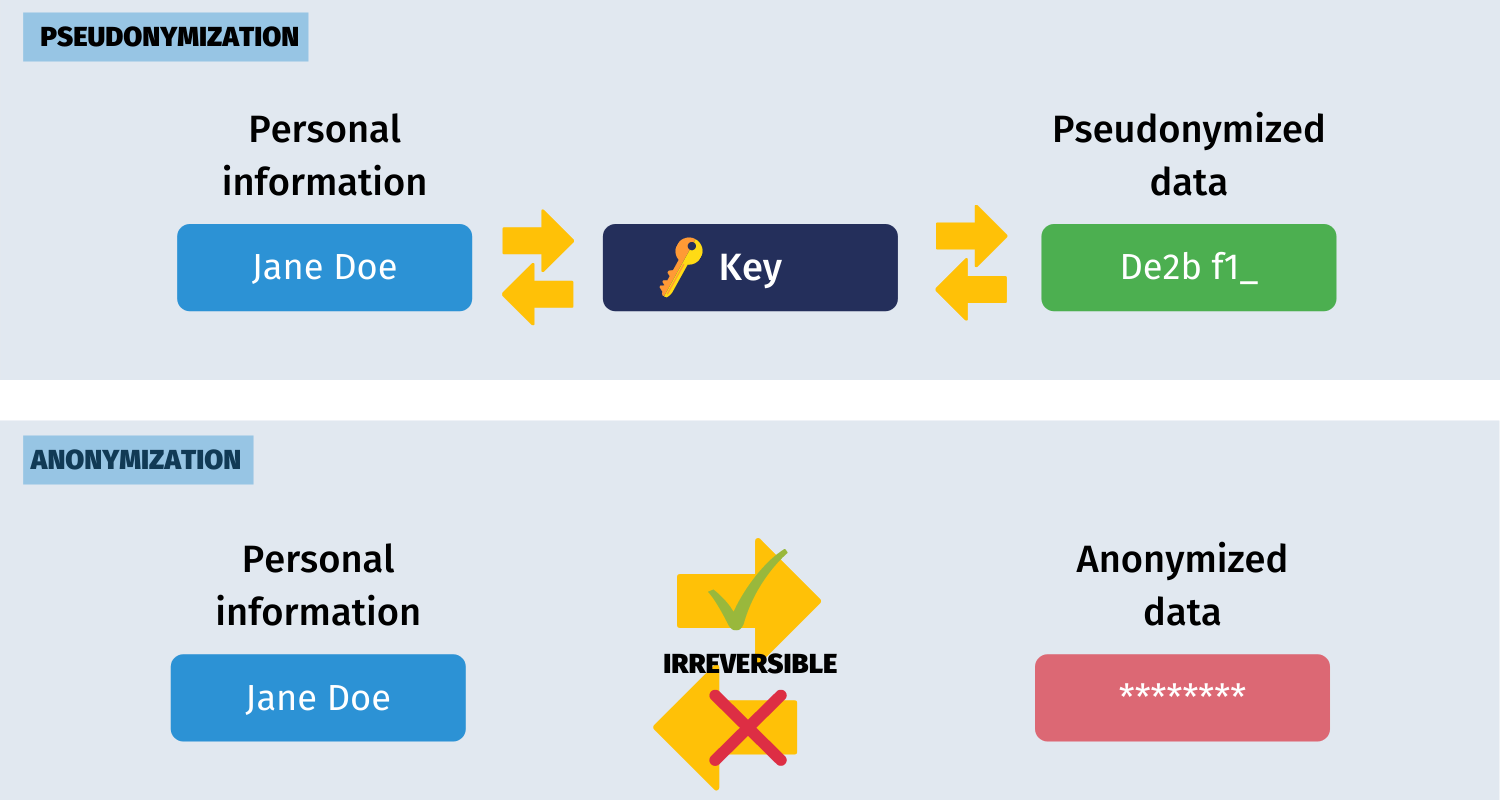
\includegraphics[width=0.8\linewidth]{Images/Difference-between-anonymization-and-pseudonymization.png}
    \caption{Pseudonimizzazione VS Anonimizzazione}
    \label{fig:enter-label}
\end{figure}
